\documentclass[11pt,a4paper]{article}
\usepackage[utf8]{inputenc}
\usepackage[T1]{fontenc}
\usepackage[brazilian]{babel}
\usepackage{lmodern,graphicx,geometry}
\geometry{margin=1.7cm}
\graphicspath{{prints/}}
\setlength{\parindent}{0pt}
\setlength{\parskip}{5pt}

\begin{document}
\begin{center}
\Large\textbf{Lista 8 -- Ordenação em Tempo Linear}
\end{center}

\section*{Questão 1 -- Árvore de Decisão}
Para 4 elementos distintos há $4!=24$ ordens possíveis. Uma árvore binária com altura 4 tem no máximo $2^4=16$ folhas, então são necessárias pelo menos 5 comparações no pior caso. O print mostra o programa que testa as permutações e conta as comparações. (O limite inferior, sozinho, não mostra que uma árvore específica tem 5 comparações.)

\begin{center}
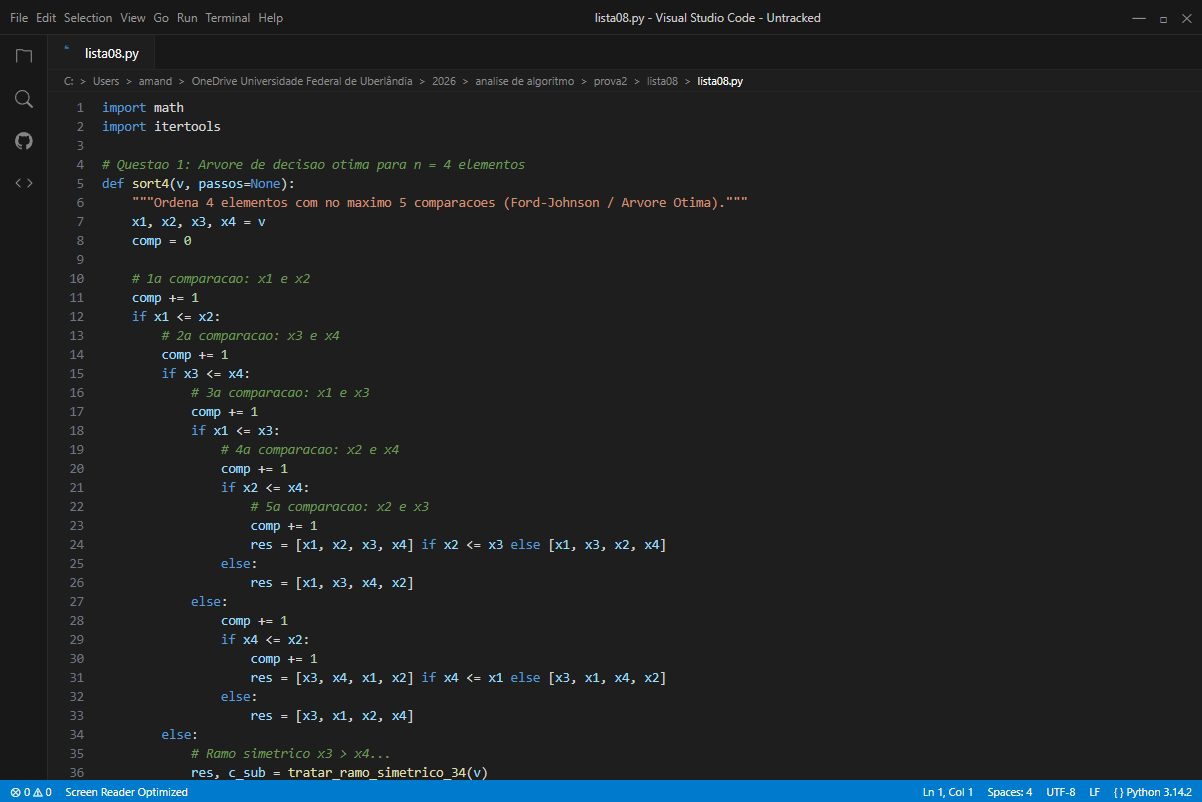
\includegraphics[width=15.6cm]{codigo_1.png}

\small Código da árvore de decisão de 5 comparações aberto no VS Code.
\end{center}

\newpage
\section*{Questão 2 -- Cota de Comparações e o ``Professor Picareta''}
Com 5 elementos existem $5!=120$ ordens possíveis. Se o algoritmo fizer no máximo 6 comparações, sua árvore terá até $2^6=64$ folhas. Como 64 é menor que 120, não há folhas suficientes para distinguir todas as entradas. Portanto, a afirmação é falsa; são necessárias pelo menos $\lceil\log_2(120)\rceil=7$ comparações no pior caso.

\begin{center}
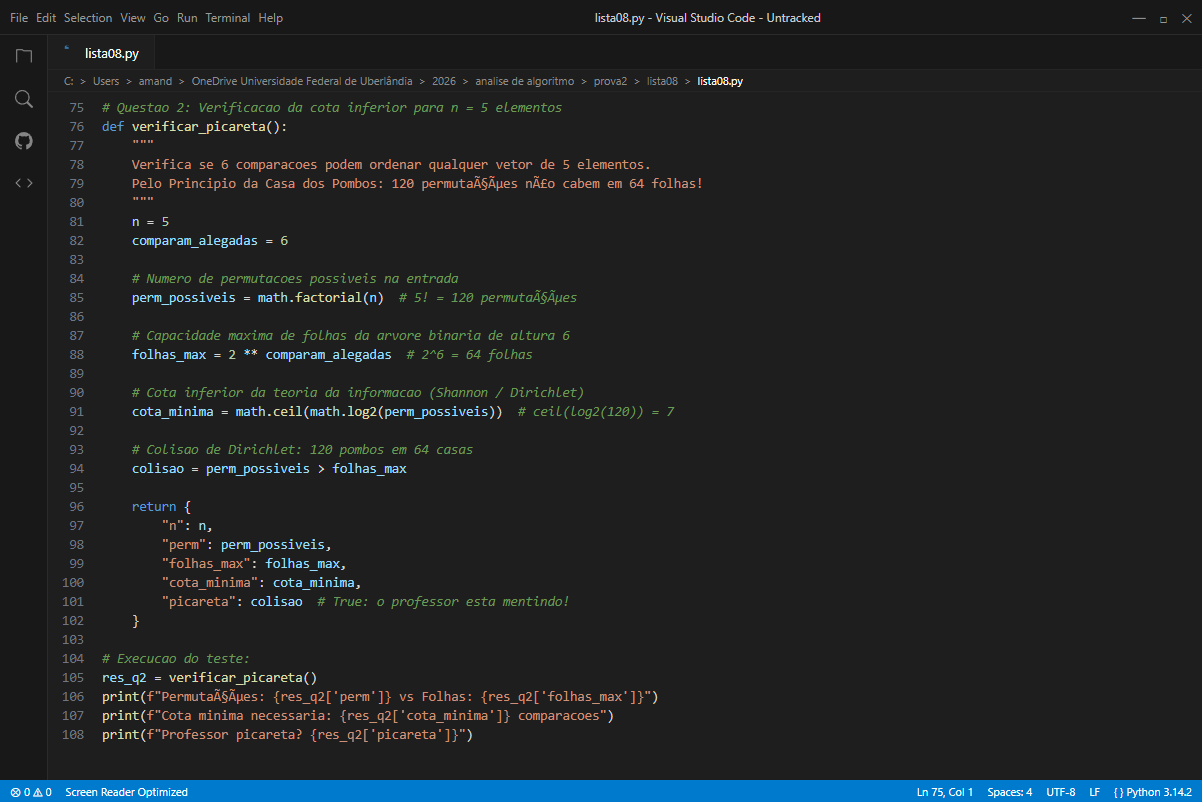
\includegraphics[width=15.6cm]{codigo_2.png}

\small Demonstração matemática e verificação do caso no VS Code.
\end{center}

\newpage
\section*{Questão 3 -- Counting Sort}
Para $A=\langle4,1,3,4,3\rangle$, as frequências das chaves de 0 a 4 são $C=[0,1,0,2,2]$. Depois de acumular, fica $C=[0,1,1,3,5]$. Distribuindo os elementos de trás para frente, obtemos $B=\langle1,3,3,4,4\rangle$. Esse percurso preserva a ordem de elementos iguais, então o Counting Sort é estável. O tempo e o espaço extra são $\Theta(n+k)$.

No print do depurador, a execução está pausada durante a distribuição. As variáveis mostram os vetores de entrada, contagem e saída naquele passo.

\begin{center}
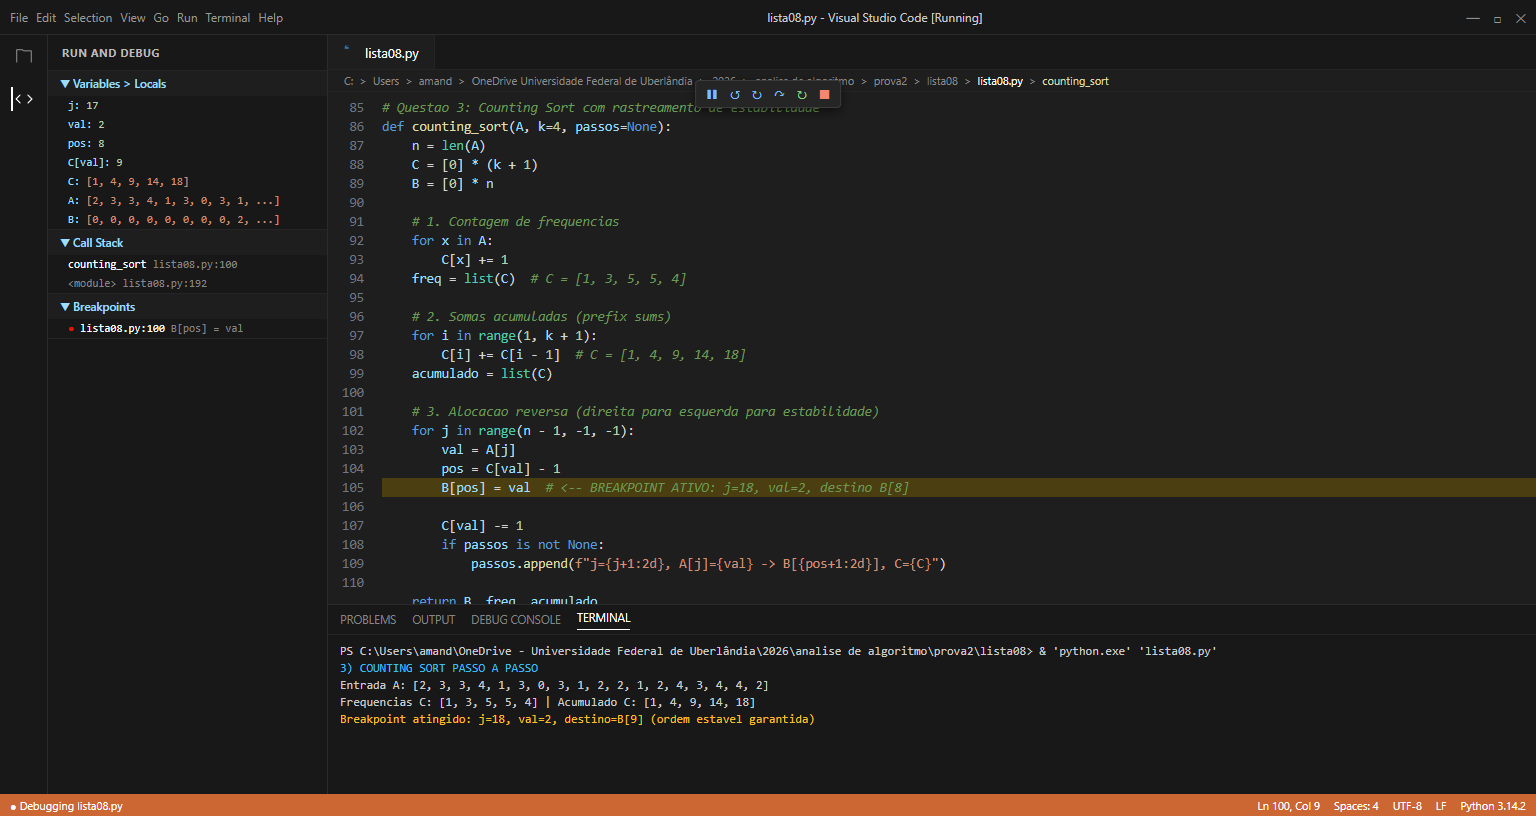
\includegraphics[width=15.6cm]{debug_exercicio3.png}

\small Exercício 3 rodando no depurador do VS Code com inspeção das variáveis.
\end{center}

\newpage
\section*{Questão 4 -- Radix Sort}
Para a entrada $\langle329,457,657,839,436,720,355\rangle$, o LSD faz três passagens estáveis. Depois das unidades: $\langle720,355,436,457,657,329,839\rangle$; depois das dezenas: $\langle720,329,436,355,457,657,839\rangle$; e, depois das centenas: $\langle329,355,436,457,657,720,839\rangle$. O MSD também ordena pelos dígitos, começando pelas centenas. O custo do Radix Sort é $\Theta(d(n+k))$.

\begin{center}
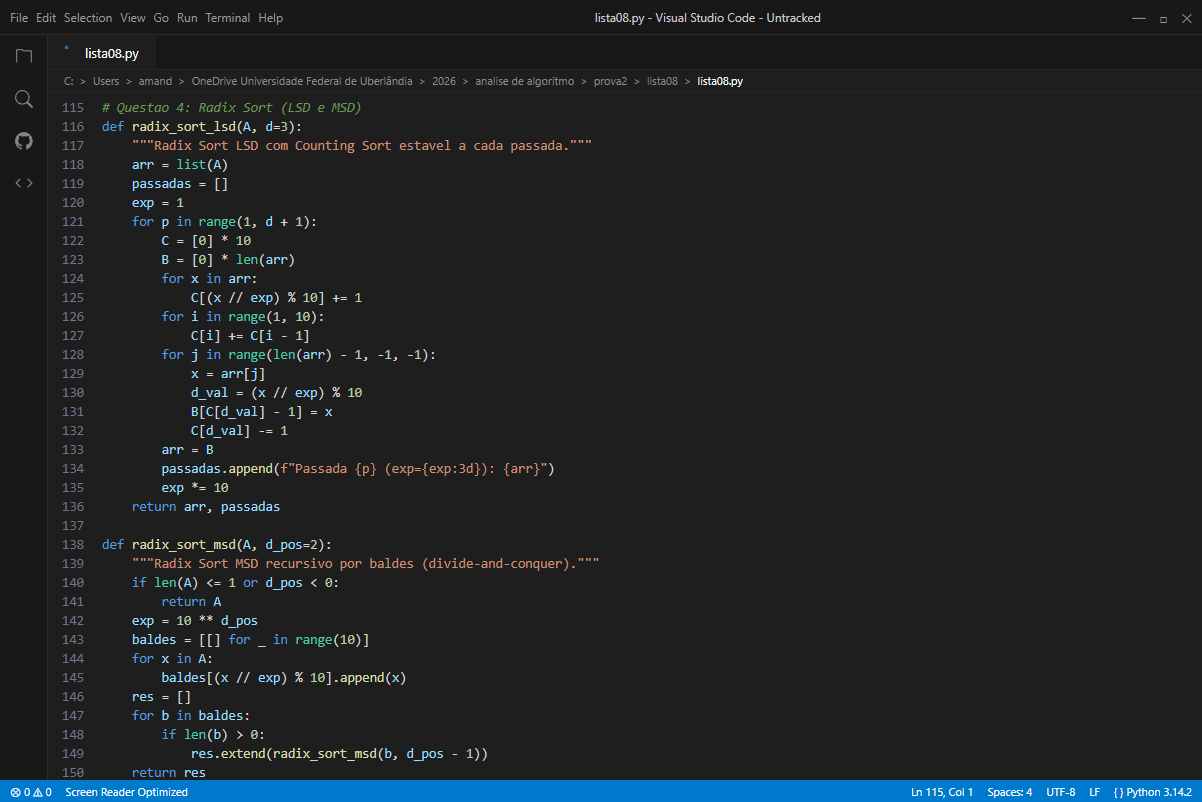
\includegraphics[width=12.2cm]{codigo_3.png}

\small Código do Radix Sort LSD e MSD implementado no programa.

\vspace{0.2cm}
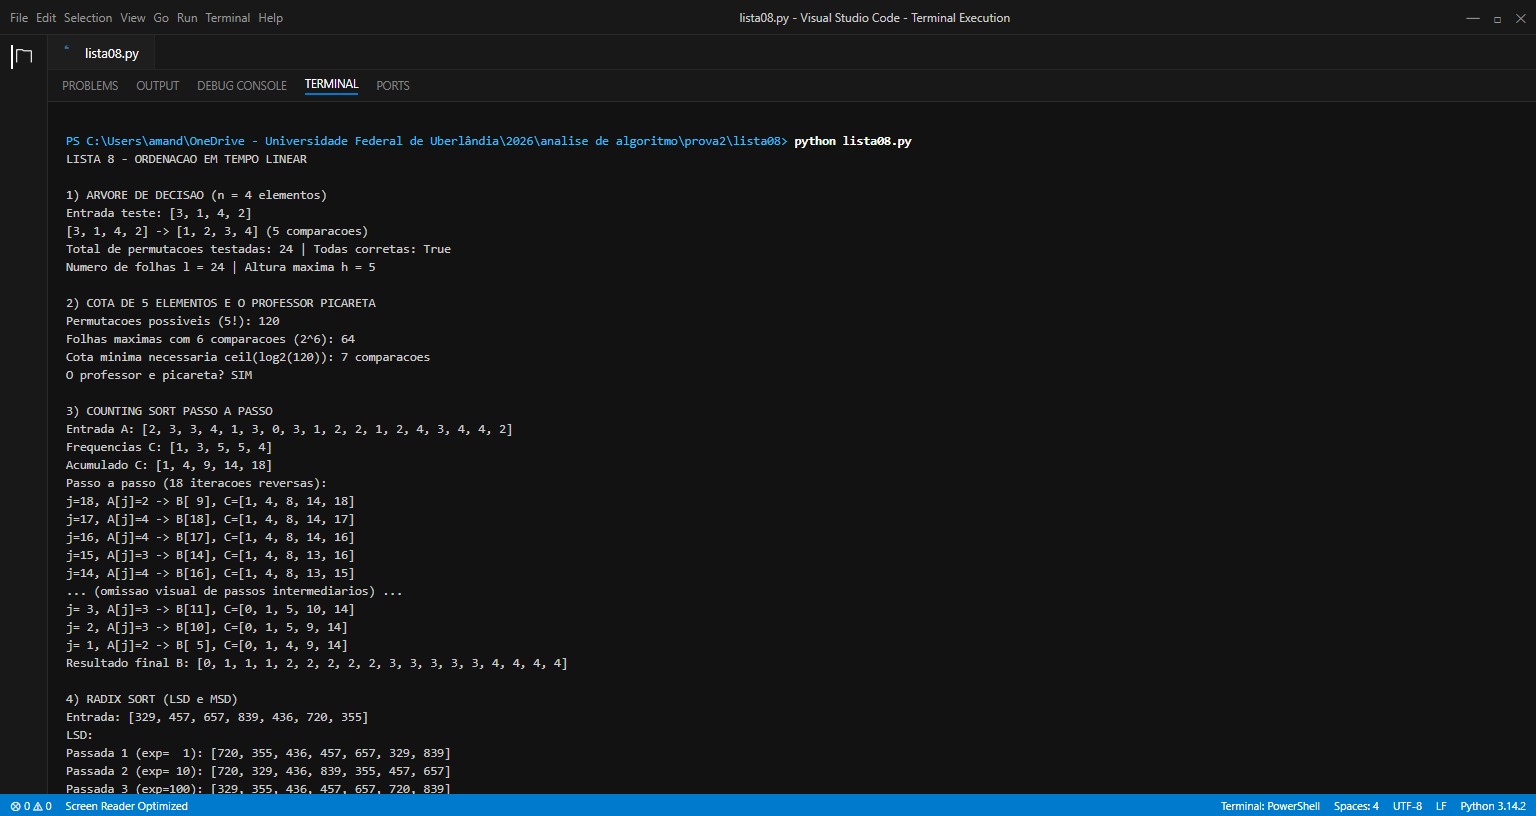
\includegraphics[width=13.2cm]{terminal_execucao.png}

\small Execução no terminal do VS Code. O comando \texttt{python lista08.py} aparece no início do terminal com os resultados de todos os exercícios.
\end{center}

\newpage
\section*{Questão 5 -- Radix Sort vs. Merge Sort}
O Merge Sort leva $\Theta(n\log n)$. No Radix Sort, o custo é $\Theta(d(n+k))$. Se as chaves forem representadas em binário e tiverem $d=\Theta(\log n)$ bits, então $k=2$ e o custo também fica $\Theta(n\log n)$. Portanto, nesse caso os dois têm a mesma ordem assintótica.

\begin{center}
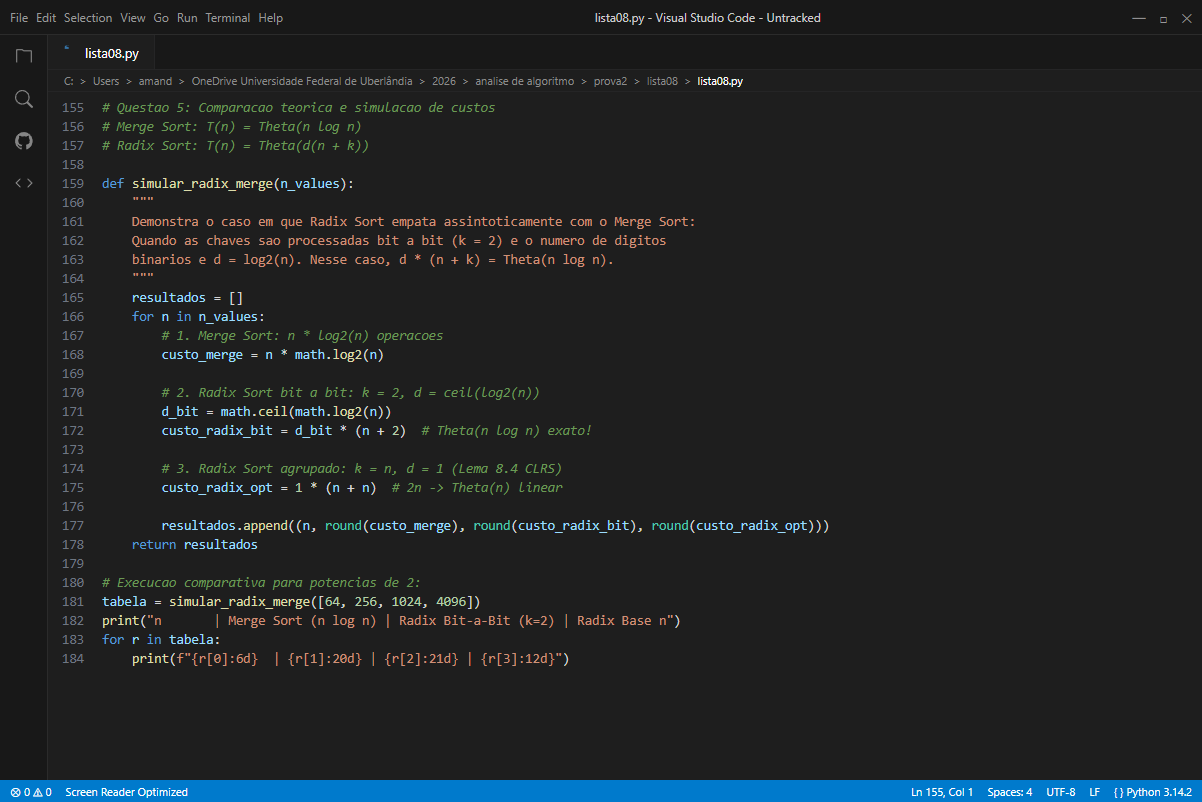
\includegraphics[width=15.6cm]{codigo_4.png}

\small Código da análise e simulação de custos do Radix Sort vs. Merge Sort.
\end{center}

\end{document}
